% !TEX root = main.tex
\section{Literature review}\label{sec:literature}

This section will consist of research papers focused on these main topics: 
\begin{itemize}
    \item \textit{Ranking static analysis alerts}: some of the most known (cited) approaches to rank alerts.
    \begin{itemize}
        \item Using a single SA tool
        \item Combining multiple tools
        \item Looking at survey papers that describe the state of the research and state of the art techniques.
        \item Comparative studies evaluating different methods.
    \end{itemize}
    \item \textit{Bug prediction}: Rank the alerts in problematic parts of code higher.
    \item Information on \textit{real world usage of SA tools}, problems and suggested solutions.
\end{itemize}

 \subsection{Dealing with False Positives}

 \subsubsection{Single Tool}

 Kremenek and Engler \cite{z-ranking} introduce \textit{Z-ranking}, a statistical model to rank the error reports of SA tools. They make a distinction between successful and failed checks (those that satisfy a checked property and those that violate it). The underlying observation is that the most reliable error reports are those that generated few failed checks and many successful checks, since the actual amount of bugs in code is relatively small. An explosion of failed checks is a likely indicator that something is going wrong with the analysis. Reports are sorted based on the calculated \textit{z-test} statistic (based on the relative frequency of successful and failed checks).

 The problem can be formally defined as a classification task. Let P be the population of all reports, both successful checks and failed checks, emitted by a program checker analysis tool. \textit{P} consists of two subpopulations: \textit{S}, the subpopulation of successful checks and \textit{E}, the subpopulation of failed checks (or error reports). The set of error reports \textit{E} can be further broken down into two subpopulations: \textit{B}, the population of true errors or bugs and \textit{F}, the population of false positives. The classification problem can then be restated as follows: given an error report $x \in E$, decide which of the two populations \textit{B} and \textit{F} it belongs to. That is based on the fact that \textit{B} and \textit{F} have different statistical characteristics. 

 Given a grouping operator \textit{G} that groups successful and failed checks together, we calculate the proportion of failed checks $G.\rho = \frac{G.successful}{G.failed}$. Populations are ranked both by the $\rho$ value and by the degree of confidence in its estimation. By treating these checks inside the groups as a sequence of binary trials (coin tosses). The probability $p_i$ of success will have to be approximated using the standard error. By using the \textit{z-test} statistic, which measures how far an observed value is from the real population, a value can be specified that produces a large positive \textit{z-score} when there are few errors and many successes, and a large negative \textit{z-score} when there are few successes and many errors.

 Given an estimated $p_i$ and a calculated \textit{SE}, we can chose $p_0$ to produce the effect mentioned above:
 $z=\frac{observed-expected}{SE}=\frac{p_i-p_0}{SE}=\frac{p_i-p_0}{\sqrt{\frac{p_0(1-p_0)}{n}}}$. The average population success rate can be chosen as a starting point for the value of $p_0$.

 According to their tests, \textit{Z-ranking} performed better than randomized ranking 98.5\% of the time. Moreover, within the first 10\% of reports inspected, \textit{Z-ranking} found 3-7 times more real bugs on average than found by randomized ranking.\\

 \begin{figure}[H]
     \begin{subfigure}{1\textwidth}
         \centering
         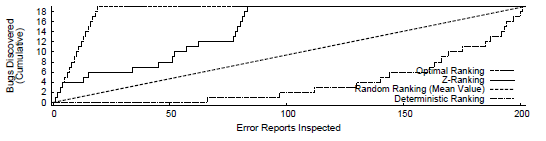
\includegraphics[scale=0.7]{./src/z_ranking_result_linux_intra.png}
         \caption{Intra-procedural check on Linux spin (lock)}
     \end{subfigure}\\
     \begin{subfigure}{1\textwidth}
         \centering
         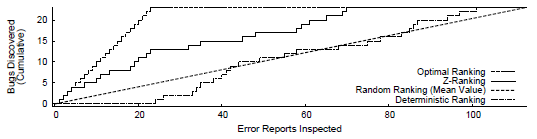
\includegraphics[scale=0.7]{./src/z_ranking_result_linux_inter.png}
         \caption{Inter-procedural check on Linux (free calls)}
     \end{subfigure}
 \end{figure}


 Kremenek et al. \cite{correlation_exploitation} introduce \textit{Feedback-Rank}, a dynamic ranking scheme that adapts as reports are inspected. By analyzing historical data, they observed that both bugs and false positives cluster by code locality. They present a probabilistic technique that exploits this correlation and also incorporates user feedback by reordering reports after each inspection. Since reports are correlated within a population (cluster), inspecting one of them yields information about the others. The ranking works by using a \textit{Bayesian Network} and exploiting two features, the number of populations (error messages grouped together) and the strength of correlation in each population. Furthermore, the strategy also continues improving with time, by taking into account the history of inspections.

 An intuitive explanation for the reason that reports cluster is given for both real and false positives. Regarding true positives, when developers do not know a rule, they will repeatedly violate it, so errors of the same type will correlate together. As for the false positives, there are three main causes: analysis mistakes of the tool (explosion of errors), rare coding idioms used by developers (which trigger the tools), incomplete rule specifications (a rule holds in most cases, but can be safely violated in others).

 To cluster the reports, code locality in different granularities is chosen: function, file and directory level. From the results in \cref{fr:lshape} it can be seen that very few populations contain a mix of bugs and false positives. \textit{Applicability} is defined as the ratio of non singleton clusters (which are bad for online ranking) to the total amount of clusters. The coarser the granularity the greater the applicability but also the smaller the correlation. \textit{Skew} is defined as the ratio of homogeneous clusters (all bugs or all false positives) to the total number of clusters. In this case, the more refined the granularity (function level), the higher the skew. Thus, a trade-off needs to be made between applicability and skew.

 To apply the algorithm a model is needed that produces the correlations among the reports. The reports are divided into two major regions, one that contains mostly true positive ($g_B$), and one that contains mostly false positives ($g_{FP}$) (see \cref{fr:partition}). A \textit{Bayesian Network} is used to calculate the probabilities of a cluster belonging to a certain region (regions are different for different granularities). The initial configuration can either be chosen by the user or learned from historical data. A simple model can be seen on \cref{fr:bayes}, where 3 reports depend on the probabilities of the parent function, file and directory clusters they belong to. Influence though, flows across both directions: if we inspect a report and know its value, the probabilities of the parents are re-calculated. Gives a training set, the conditional probability distributions of the network (along with the probabilities for the regions) can be learned using \textit{Expectation Maximization}. \textit{Belief Propagation} is used to update probabilities after each inspection and \textit{Information Gain} is used as a secondary factor to rank the reports. 

 Feedback-Rank represents a complementary approach to static ranking schemes (it can be combined with Z-Ranking for example) and can be trained with other forms of correlation instead of code locality. 

 According to their tests, \textit{Feedback-Rank} performed 2-8 times better than randomized ranking.\\

 \begin{figure}[H]
     \begin{subfigure}{1\textwidth}
         \centering
         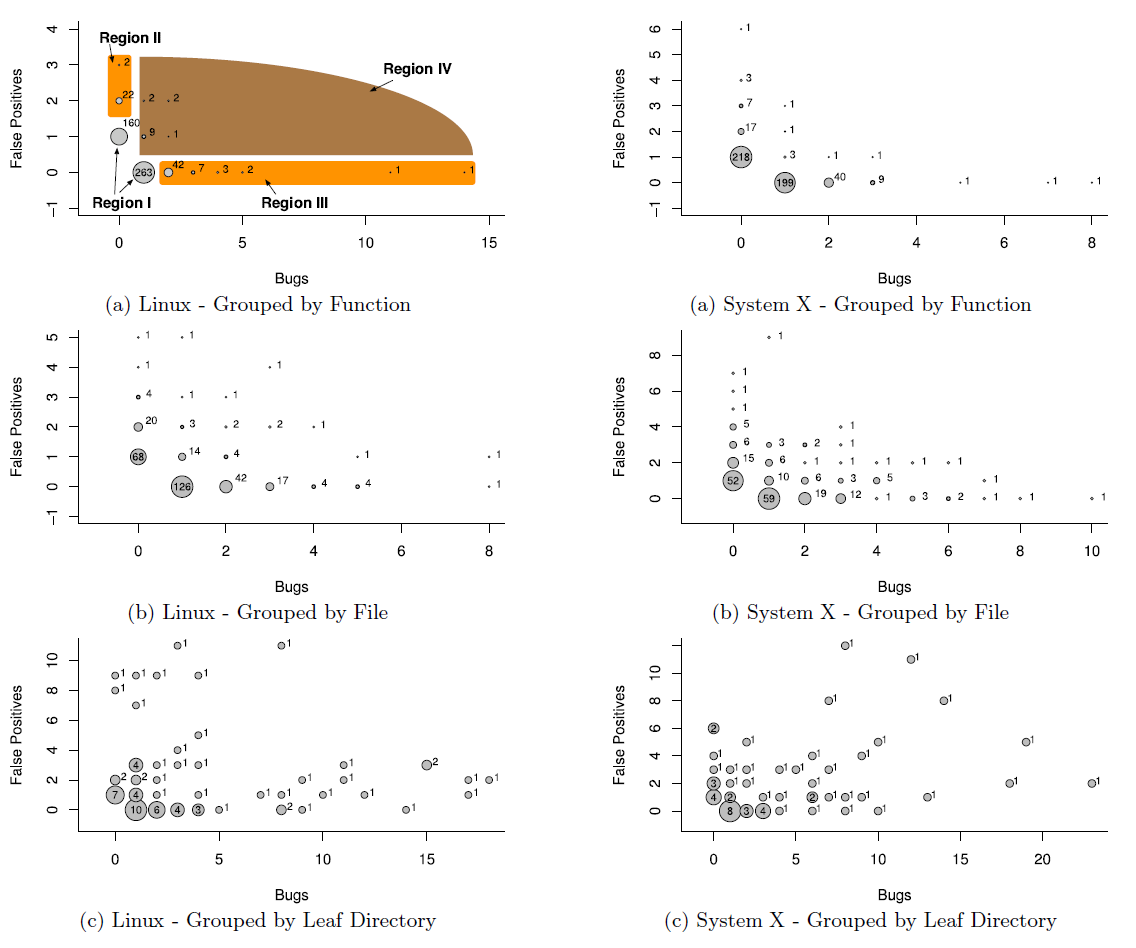
\includegraphics[scale=0.4]{./src/feedback_rank_l_shape.png}
         \caption{"L" shape of clustering}\label{fr:lshape}
     \end{subfigure}\\
     \begin{subfigure}{.5\textwidth}
         \centering
         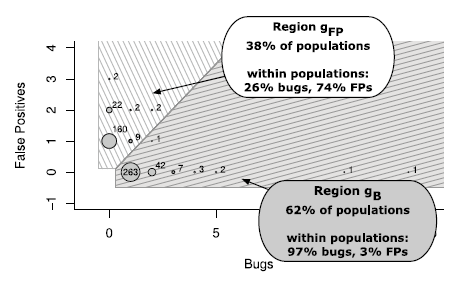
\includegraphics[scale=0.6]{./src/feedback_rank_partition.png}
         \caption{Populations divided into regions, mostly true or false positives}\label{fr:partition}
     \end{subfigure}%
     \begin{subfigure}{.7\textwidth}
         \centering
         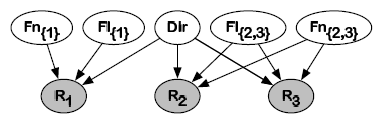
\includegraphics[scale=0.4]{./src/feedback_rank_bayes.png}
         \caption{Sample Bayesian network with 3 reports}\label{fr:bayes}
     \end{subfigure}
 \end{figure}


 Boogerd and Moonen \cite{static_profiling} present a technique, \textit{ELAN}, that prioritizes SA warnings by using the (predicted) likelihood that the execution reaches the location for which the warnings are reported. The execution likelihood is defined as the probability that a program point will be executed at least one in an arbitrary program run and is calculated statically. This computation is demand-driven, thus it is only performed for the locations associated with warning reports.

 The workflow (\cref{elan:workflow}) consists of normalizing the results of SA tools (to a specific format), creating system dependency graphs, calculating for every warning the likelihood of execution, ordering the results using the execution probability and possibly other external techniques (like Z-Ranking). 

 Likelihood analysis is based on system dependency graphs, which tie all program dependency graphs (function level) together by modelling the inter-procedural control dependencies. Their approach only considers control flow and ignore dataflow information. In order to avoid traversing all the SDG, \textit{program slicing} is used on control points. Other than the basic algorithm, they also introduce branch prediction heuristics, which do not excessively impact performance.

 Experiments show that predicted execution likelihoods correlate with data extracted from dynamic profiling. One problem though, is that when for example 30\% of all code is always executed, then the ranking of those warnings that belong to that piece of code, cannot be distinguished.

 \begin{figure}[H]
     \centering
     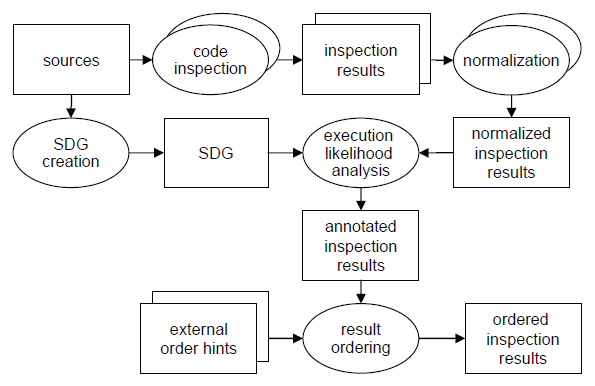
\includegraphics[scale=0.4]{./src/elan_workflow.png}
     \caption{Workflow for the ELAN tool}\label{elan:workflow}
 \end{figure}


 Kim and Ernst \cite{which_warnings} propose a history-based warning prioritization (HWP) algorithm which works by mining fix-changes in the VCS. It is based in the intuition that if a warning is removed by a fix, then probably that warning was important. On the other hand, if a warning instance is not removed for a long time, then warnings of
 that category may be neglectable, since the problem was not noticed or was not considered worth fixing. They measured the tool warning prioritization (TWP) on three different systems and found a precision of 3\%, 12\% and 8\%.  

 They set a weight to each warning category to represents its importance. The weight will be proportional to the number of warnings eliminated by changes (where fix-changes have the biggest weight, \cref{which_warnings:weights}). Selecting the top weighted warnings improves precision up to 17\%, 25\%, and 67\% respectively. Precision is calculated as $precision = \frac{number\:of \:warnings\:on\:bug\:related\:lines}{total\:number\:of\:warnings}$.
 By looking at the fix-changes and corresponding affected lines, by starting at the last revision, they can mark the bug-related lines, up to the first revision when they appeared (\cref{which_warnings:marking}). Ranking is category-based, so only the categories of warnings are considered and there is no distinction between the warnings inside each category. The algorithm works well if the categories are fine grained and internally homogeneous.

 They measure precision by training the weights in the first half of the version history, and testing them on the other half. The HWP outperforms TWP for all three systems (\cref{which_warnings:results}).

 \begin{figure}[H]
     \begin{subfigure}{0.6\textwidth}
         \begin{subfigure}{.5\textwidth}
             \centering
             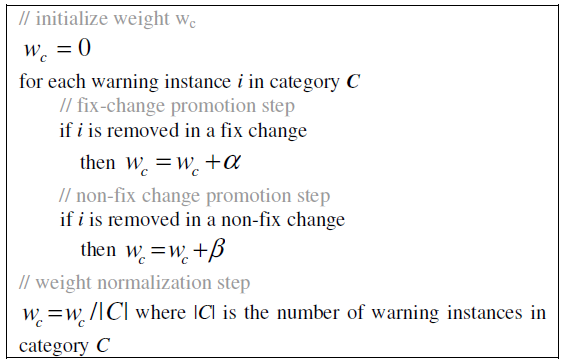
\includegraphics[scale=0.45]{./src/which_warnings_weights.png}
             \caption{Precision results at line-level}\label{which_warnings:weights}
         \end{subfigure}\\
         \begin{subfigure}{.5\textwidth}
         \centering
         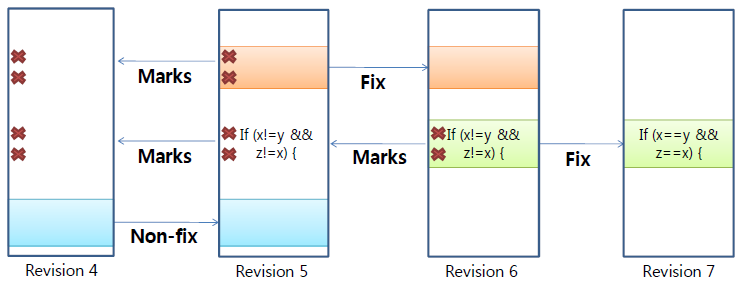
\includegraphics[scale=0.35]{./src/which_warnings_marking.png}
         \caption{Line marking approach}\label{which_warnings:marking}
         \end{subfigure}
     \end{subfigure}%
     \begin{subfigure}{0.4\textwidth}
         \centering
         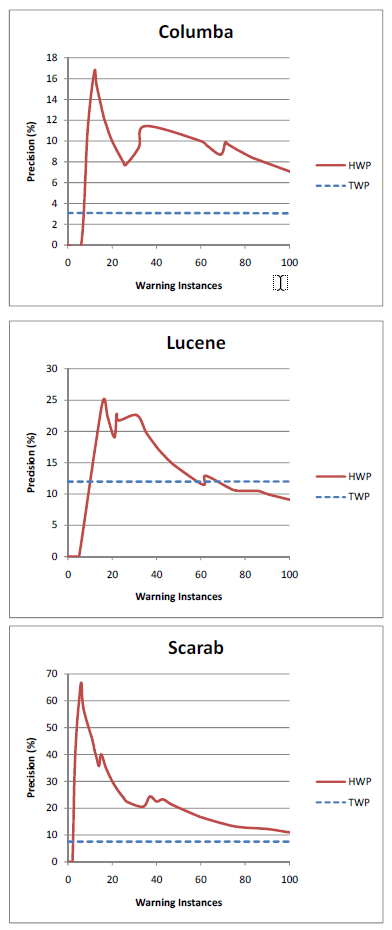
\includegraphics[scale=0.5]{./src/which_warnings_results.png}
         \caption{Line marking approach}\label{which_warnings:results}
     \end{subfigure}
 \end{figure}


 Ruthruff et al. \cite{actionable_sa} use \textit{logistic regression} models to not only reduce the number of false positives in the output of SA tools, but also to predict actionable warnings. Warnings are not always acted on by developers even if they reveal true defects. The reason may be that the defects may have little impact and require significant effort for little perceived benefit. Furthermore, they introduce a statistical methodology for discarding features with low predictive power and thus avoiding the capture of expensive data. Information to build the models is mainly drawn from: (a) light-weight code complexity metrics for post-release bug prediction, (b) file (history) information to predict fault counts within individual files. The features include the history of warnings, source code characteristics, churn factors, and warnings descriptors (\cref{act:metrics}).

 Their screening methodology, for selecting an independent subset of predictor features, consists of up to four stages, and attempts to identify at least six predictive features. The stages respectively consider 5\%, 25\%, 50\%, 100\% of the warnings, continuously removing features with low predictive power. One of the reasons to consider this cost-effective approach is that it may be desirable to rebuild the models at different points in time, either because a significant number of new warnings have been reported, or the codebase has undergone substantial change.

 By considering a sample of around 1600 warnings (inspected by two engineers), and by using different models (with resulting different features) for classifying true positives and actionable warnings, they achieved an accuracy of 85\% for the former, and 70\% for the later (\cref{act:results}).

 \begin{figure}[H]
     \begin{subfigure}{.5\textwidth}
         \centering
         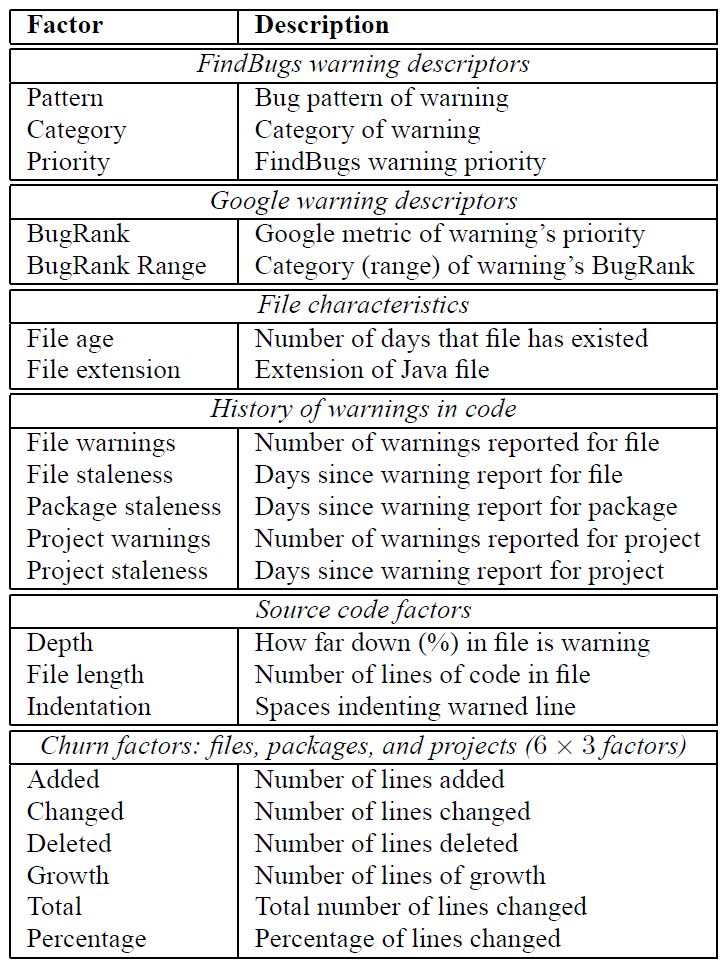
\includegraphics[scale=0.3]{./src/actionable_warnings_metrics.png}
         \caption{Some of the features considered for building the models}\label{act:metrics}
     \end{subfigure}%
     \begin{subfigure}{.5\textwidth}
         \centering
         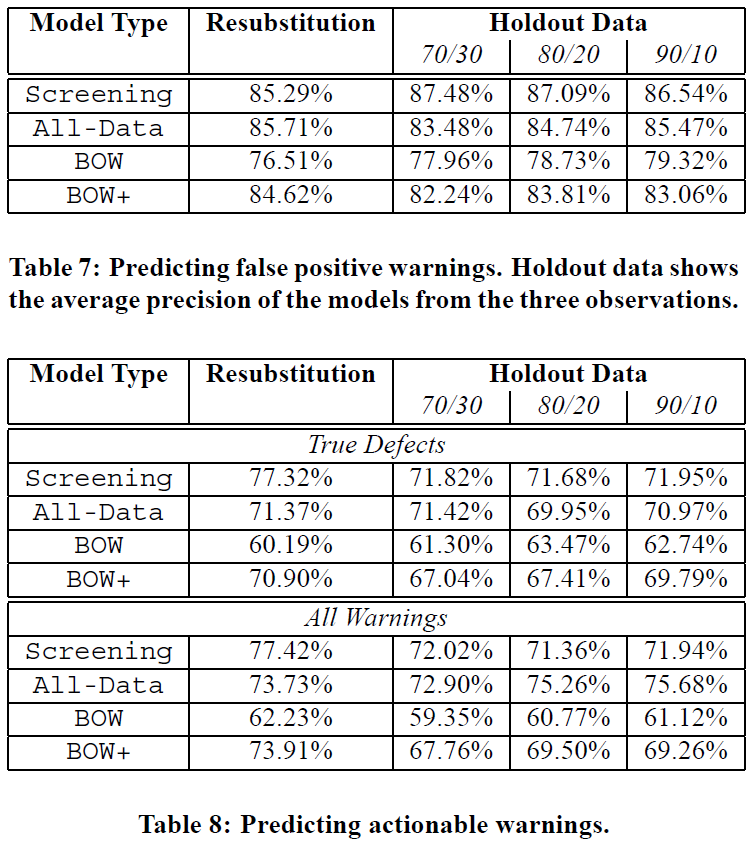
\includegraphics[scale=0.3]{./src/actionable_warnings_results.png}
         \caption{Results for predicting true positives and actionable warnings}\label{act:results}
     \end{subfigure}
 \end{figure}


 Hanam et al. \cite{alert_patterns} present a method for differentiating actionable and unactionable alerts by finding alerts with similar code patterns (alerts with similar patterns are probably of the same type). They use a feature vector based on code characteristics at the site of each SA alert along with a classifier to build a model for predicting AA. They introduce the notion of \textit{alert patterns}, source code patterns employed by developers that are unactionable but are repeatedly flagged by SA tools (or similarly always actionable).

 To extract features from the site of the warning (and near it), lightweight program slicing is used. Backwards slicing is used to detect which statements could have affected the outcome of the seed statement (place of the alert). To speed up the slicing process, all external classes are excluded from the analysis and the depth is limited to the 5 nearest statements prior to the seed.

 By using the source code history of three projects to train and test their approach, they achieve considerably better results than the default ranking of a SA tool (57 vs 19 AA in the top 20\% of the alert list), and a slight improvement (6\%) than the existing techniques.

 \begin{figure}[H]
     \begin{subfigure}{.5\textwidth}
         \centering
         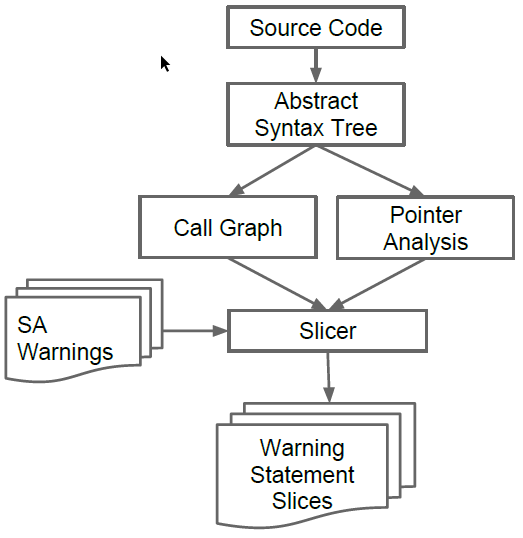
\includegraphics[scale=0.3]{./src/alert_patterns_slicing.png}
         \caption{Method for generating slices}\label{alert_patterns:slicing}
     \end{subfigure}%
     \begin{subfigure}{.5\textwidth}
         \centering
         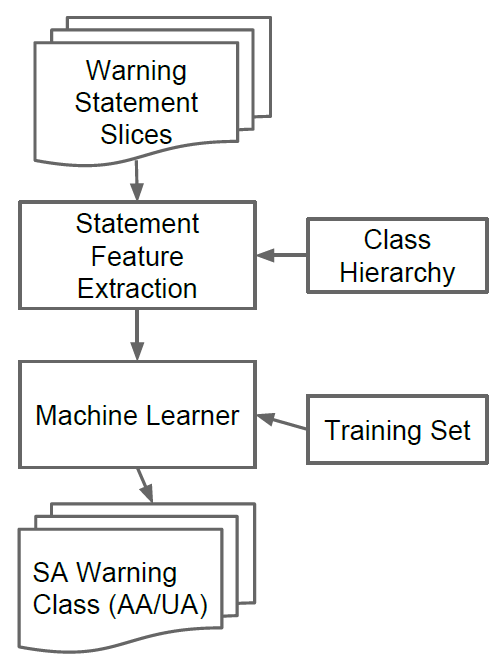
\includegraphics[scale=0.3]{./src/alert_patterns_workflow.png}
         \caption{Workflow for classifying alerts}\label{alert_patterns:workflow}
     \end{subfigure}
 \end{figure}


 Venkatasubramanyam and Gupta \cite{incremental_sa} propose an incremental and lightweight approach to detect coding violations by using a learning system. They track warnings through the version history to detect patterns and determine which SA rules are important (and must be enabled). Their approach focuses on differential code analysis (filter/identify violations happening only on new parts of code), and on learning from the experts.

 Their methodology (\cref{incremental_sa:workflow}) consists of database that continuously stores information about SA rules. The initial version is build by mining (at least) the last three version of the software under analysis. To train the classifier (learning system) different features are used: patterns of code where SA violations are reported, impact of the violations on code quality, confidence level of the rules (probability that a rule gives a false positive), most commonly committed errors (reflecting the developers pattern of coding) and the most recently committed errors.

 New code changes made by developers are checked against the database. By using a patterns matching algorithm that compares new code with the patterns saved in the database, possible bugs can be detected. This approach potentially permits to run the SA tools less frequently, since code violations can be suggested by comparing against past saved patterns. They also suggest using \textit{first order logic} for capturing the context around rule violations and thus learning what factors produce a false/true positive.

 \begin{figure}[H]
     \centering
     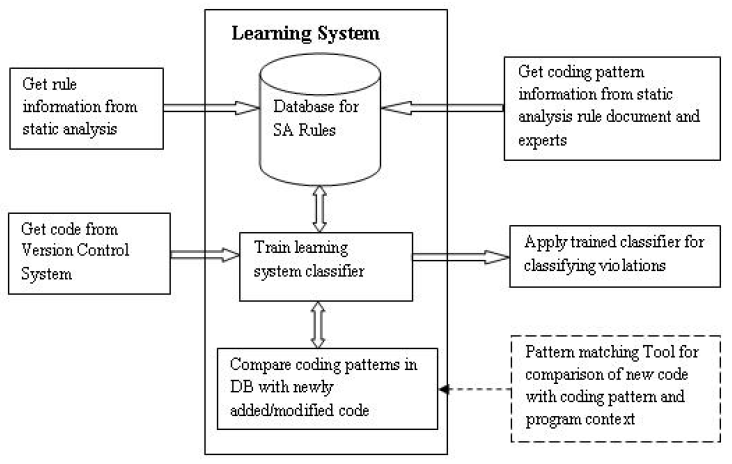
\includegraphics[scale=0.3]{./src/incremental_sa_workflow.png}
     \caption{Workflow for incremental violation detection}\label{incremental_sa:workflow}
 \end{figure}


 Heckman and Williams \cite{model_building_actionable} present a generic approach for building actionable alert machine learning models and provide a comparative study of different algorithms tested of two Java systems. Their initial feature set consists of 51 alert characteristics originating from alert type and history, software metric, software history and source code churn.

 To collect data, they check out and build the program for each chosen revision (in practice they did that once in every 25 revisions) and collect alerts and their characteristics. Starting from the first revision, the sets of alerts between two revisions are compared, collecting information when alerts are opened and closed (and thus classifying them as actionable or unactionable).

 By trying different feature reduction strategies and different machine learning algorithms, they provide results for two systems. The number of selected alert characteristics ranged from 3/4 to 13/14 and both projects had 5 distinctive sets. That shows that the set of AC needs to be tailored for each project. The average metrics for all models (\cref{model_building:results}) show very good results. The difference between selected ACs and
 the best models between projects suggests that false positive mitigation models should be project-specific.

 \begin{figure}[H]
     \centering
     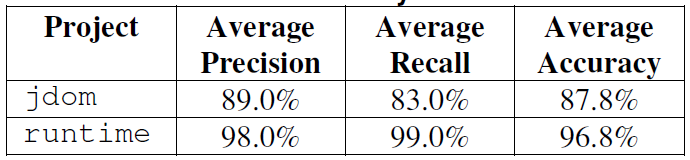
\includegraphics[scale=0.3]{./src/model_building_results.png}
     \caption{Average metrics for all models}\label{model_building:results}
 \end{figure}


 Liang et al. \cite{automatic_training_set} propose an automatic approach (\cref{automatic_training_set:workflow}) for constructing an effective training set for warning prioritization algorithms. They introduce the notion of "generic-bug-fix revisions" vs. "project-specific-bug revisions", which differentiate bug-fixing lines depending on the sort of bug that they deal with. SA tools are designed to catch generic bugs that are applicable to all projects, while most of the bugs are domain (project) specific. By restricting the training set to only those set of bugs that can be caught by the tools, models can be trained better and a higher accuracy can be reached.

 To identify generic-bug-fix revisions, they first limit the revision size to an empirically derived value (max 4 files changed). Then, they analyze the revision messages and using a natural language processing approach compare them against generic bug descriptions (by SA tools). If the similarity of these messages is above a certain threshold and the number of changed files is under the predefined limit, the revision is marked as a generic-bug-fix. To identify the generic-bug-related lines of a specific revision X, they start by analyzing all older revision than X, and backwardly calculate lines that were already present at X, when they were later changed by a generic-bug-fix revision.

 Using a \textit{K-Nearest Neighbor} classifier (trained on the first half of the revisions) paired with a feature selection algorithm, they achieve significantly better result than the tool output, especially in the first 20 warnings range. They found that using multiple SA tools gives a better result than single tool models (\cref{automatic_training_set:multiple_single}). The type training set has also an effect in the final results, models trained only with the project under analysis performed worse that models trained with extra projects (\cref{automatic_training_set:inter_intra}). That adding inter project data (at least in the case of open source projects) has a positive effect in the model predictions can be explained with the choice of focusing only on generic-bug-fix revisions.

 \begin{figure}[H]
     \begin{subfigure}{0.5\textwidth}
         \centering
         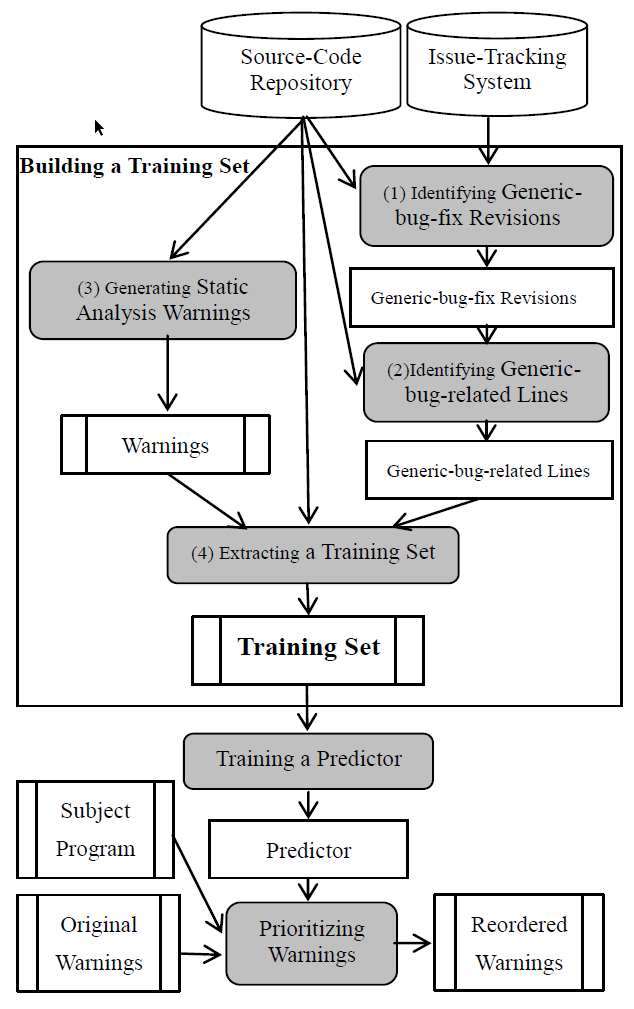
\includegraphics[scale=0.3]{./src/automatic_training_set_workflow.png}
         \caption{Workflow for constructing a training\\ set and a model}\label{automatic_training_set:workflow}
     \end{subfigure}%
     \begin{subfigure}{0.5\textwidth}
         \begin{subfigure}{.5\textwidth}
             \centering
             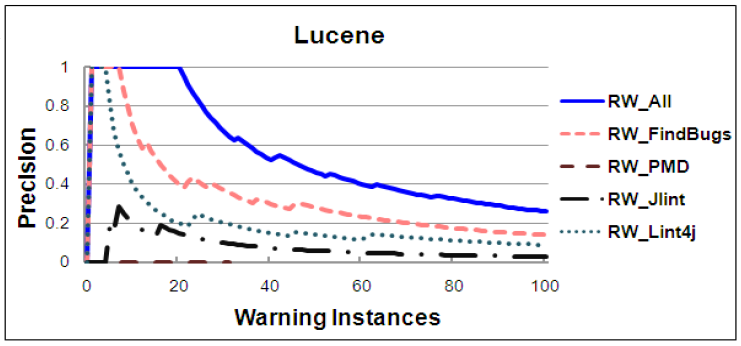
\includegraphics[scale=0.35]{./src/automatic_training_set_results1.png}
             \caption{Multiple vs. single tool results using training set}
             \label{automatic_training_set:multiple_single}
         \end{subfigure}\\
         \begin{subfigure}{.5\textwidth}
         \centering
         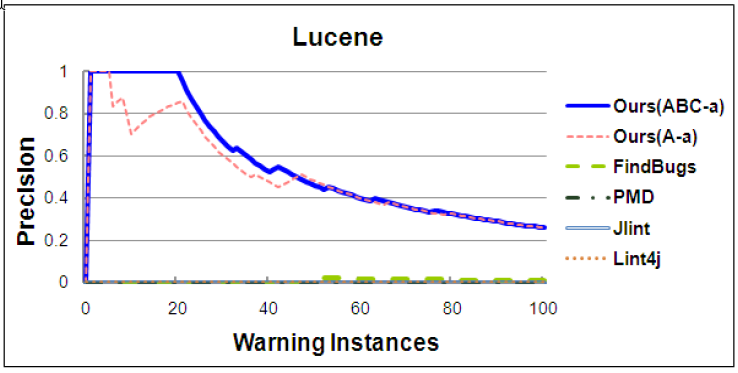
\includegraphics[scale=0.35]{./src/automatic_training_set_results2.png}
         \caption{Intra (A-a) vs inter (ABC-a) project training}
         \label{automatic_training_set:inter_intra}
         \end{subfigure}
     \end{subfigure}
 \end{figure}


 \subsubsection{Multiple Tools}

 Flynn et al. \cite{multiple_classification} use \textit{Alert Fusion} (unifying alert information from different tools) and different classifiers to classify alerts as expected true positive (e-TP), expected true negative (e-TN) and indeterminate (I). The e-TP alerts are separately prioritized for code repair and the I-alerts are automatically ranked based on classifier confidence and a cost metric to fix the code flaw. 

 The authors used a total of 354 manually audited SA alerts, which there then mapped to standardized coding rule violations (CERT). Different types of classifiers were used, using different portions of data: trained to detect a single rule violation, trained for a single programming language, and all rule classifiers. The results vary from around 80 to 90\% accuracy, depending on the classifier type. The reliability of some of the results is doubtful since one of the major problems of the study was a lack of data.

 \begin{figure}[H]
     \begin{subfigure}{.5\textwidth}
         \centering
         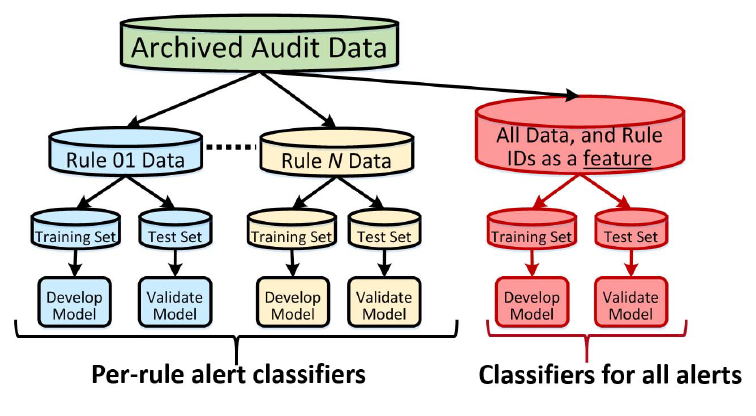
\includegraphics[scale=0.3]{./src/multiple_classifiers_workflow.png}
         \caption{Workflow of building classifiers}\label{multiple_classifiers:workflow}
     \end{subfigure}%
     \begin{subfigure}{.5\textwidth}
         \centering
         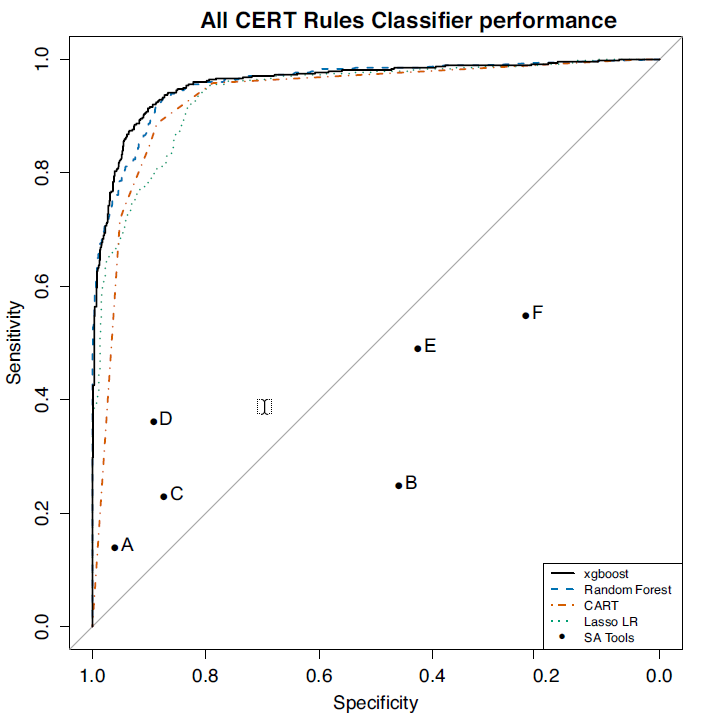
\includegraphics[scale=0.3]{./src/multiple_classifiers_resulst.png}
         \caption{Results of all-rules classifiers}\label{multiple_classifiers:results}
     \end{subfigure}
 \end{figure}


 Ribeiro et al. \cite{multiple_ensemble} aim to reduce the false positive rate of an ensemble of static analyzers by using \textit{Decision Trees} and \textit{AdaBoost}. The goal is to make possible to combine the strengths of different analyzers without suffering too much from false positives. Their approach ignores source code characteristics, making it possible to be applied without any pre-processing step on the codebase.

 They use \textit{Juliet}, a synthetic C/C++ test suite which contains specific flaws with links to program code, to train and test the classifiers (see \cref{multiple_classifiers_ensemble:warnings} for the results of different tools on the set of selected test cases). The features to train the model include the tool name, number of warnings per file, warning category, number of neighboring warnings, number of warnings per file, and a boolean feature for each of the static analyzers.

 By combining weak decision tree classifiers with AdaBoost, they can reach a mean acccuracy of 80\% with a hundred trees, with precision and recall around 68\% and 96\% respectively. The ranking is done by sorting the warnings according to the probability assigned by the model, achieving a five time improvement over random ordering. The most important features in the classifier were the number of warnings per file and the tool name.

 \begin{figure}[H]
     \begin{subfigure}{.5\textwidth}
         \centering
         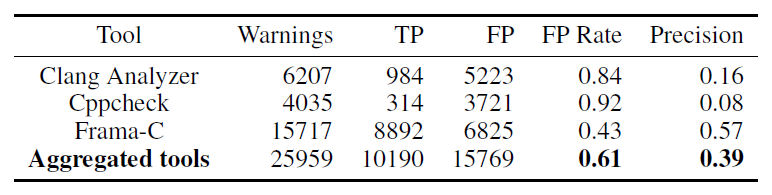
\includegraphics[scale=0.3]{./src/multiple_classifiers_ensemble_warnings.png}
         \caption{Labeled warnings per tool (from the extracted list of Juliet)}\label{multiple_classifiers_ensemble:warnings}
     \end{subfigure}%
     \begin{subfigure}{.5\textwidth}
         \centering
         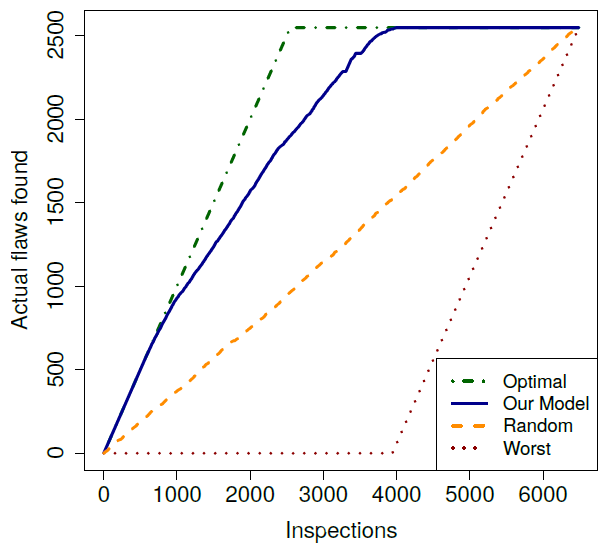
\includegraphics[scale=0.3]{./src/multiple_classifiers_ensemble_results.png}
         \caption{Results of the classifier}\label{multiple_classifiers_ensemble:results}
     \end{subfigure}
 \end{figure}


 \subsubsection{Literature review papers}

 Heckman and Williams \cite{literature_actionable} perform a systematic review of \textit{Actionable Alert Identification Techniques} (AAIT). The goal is to make an informed decision which AAIT to pair to an SA tool, in order to present relevant warnings to the tool users. An actionable alert is defined as an important, fixable anomaly. Different studies have estimated the amount of unactionable alerts ranging from 35\% to 91\%. The authors divide the tools into different categories, based on input type, approach used, and evaluation method.

 The categories of artifacts used by AAIT's are divided into five main categories: (a) alert characteristics (type, location), (b) code characteristics (metrics), (c) source code repository metrics (code churn), (d) bud database metrics, (e) dynamic analysis metrics (extracted during code execution). Most AAIT's combine more than one of these input categories.

 Approaches followed by AAIT's fall into seven main categories: (a) alert type selection (selecting altert types that are the most relevant for a codebase), (b) contextual information (limiting SA tools only to parts of code where that they can analyze well), (c) data fusion (combining multiple SA tools), (d) graph theory (system dependency graphs or repository history of changes), (e) machine learning, (f) mathematical and statistical models, (g) test case failures (generate test cases that demonstrate faults in the warning location). 

 Evaluation methodologies are divided into six categories: (a) baseline comparison (use a standard baseline), (b) benchmarks, (c) comparison to other AAIT's, (d) random and optimal order comparison, (e) train and test, (f) other.
 Classification AAIT's are evaluated using typical metrics as precision, recall, accuracy, and false positive rate, while Prioritization AAIT's are evaluated using correlation coefficients, statistical tests (chi-square), improvements over random, AUC etc..\\\\


 Muske and Serebrenik \cite{survey_approaches} perform a systematic review of SA alarm handling techniques (\cref{survey:papers}). They define \textit{handling of alarms}  as: (a) post-processing to reducing the manual inspection effort (using correlation, clustering, ranking...), and (b) supporting manual inspection of alarms.

 Seven categories for identifying alarms are defined (\cref{survey:categories}): (a) clustering, (b) ranking, (c) pruning, (d) false positive elimination, (e) combination with dynamic analysis, (f) simplifying inspections, (g) design of light-weight SA tools (\textit{LSATs}).

 In \textit{clustering}, alarms are partitioned into several groups based on similarity/correlation. There are two sub-categories: sound clustering, where there is a guarantee of certain dependencies among clustered alarms, and unsound clustering, where there are no guarantees on dependencies/relationships. 
 In \textit{ranking}, alarms are prioritized and those more likely to be errors are output at the top of the list. Different techniques can be used to support ranking, such as statistical models, history of alarm fixes, user feedback etc... 
 In \textit{pruning}, alarms are classified as actionable or non-actionable. Machine learning techniques can be used to classify the alarms (using patterns from surrounding code and syntactic/semantic differences), or alarm delta identification can be used identify the alarms that are newly generated (useful for legacy code). 
 In \textit{false positive elimination}, more precise techniques like model checking and symbolic execution are used to eliminate false positives. This approach is more precise and automatic but faces the issues of non scalability and poor performance.
 In \textit{combining dynamic and static analysis}, SA alarms are checked if they are true errors. SA has been combined with test-case generation or slicing to find errors or extract more precise information.
 In \textit{simplifying manual inspection}, approaches are used to help the user in alarm inspection by making inspections more automatic/systematic. Different techniques are used, from rule and checklist based approaches, to improved visualisation, to automatically deriving possible alarm causes.
 In \textit{designing LSATs}, light-weight, scalable and shallow analysis tools are built to avoid generation of a large number of alarms. However there are no guarantees that all defects of a type will be uncovered.

 \begin{figure}[H]
     \begin{subfigure}{1\textwidth}
         \centering
         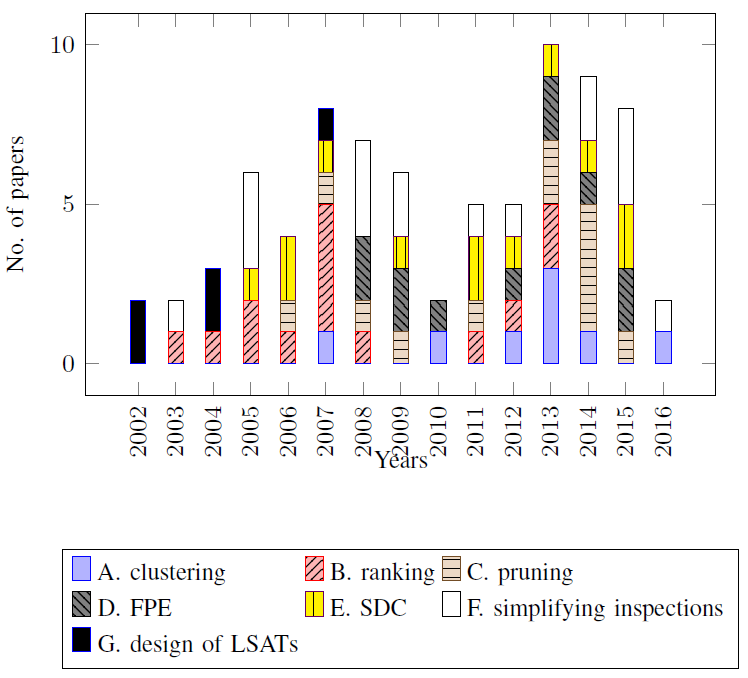
\includegraphics[scale=0.4]{./src/survey_sa_papers.png}
         \caption{Number of relevant papers per year and category}\label{survey:papers}
     \end{subfigure}\\
     \begin{subfigure}{1\textwidth}
         \centering
         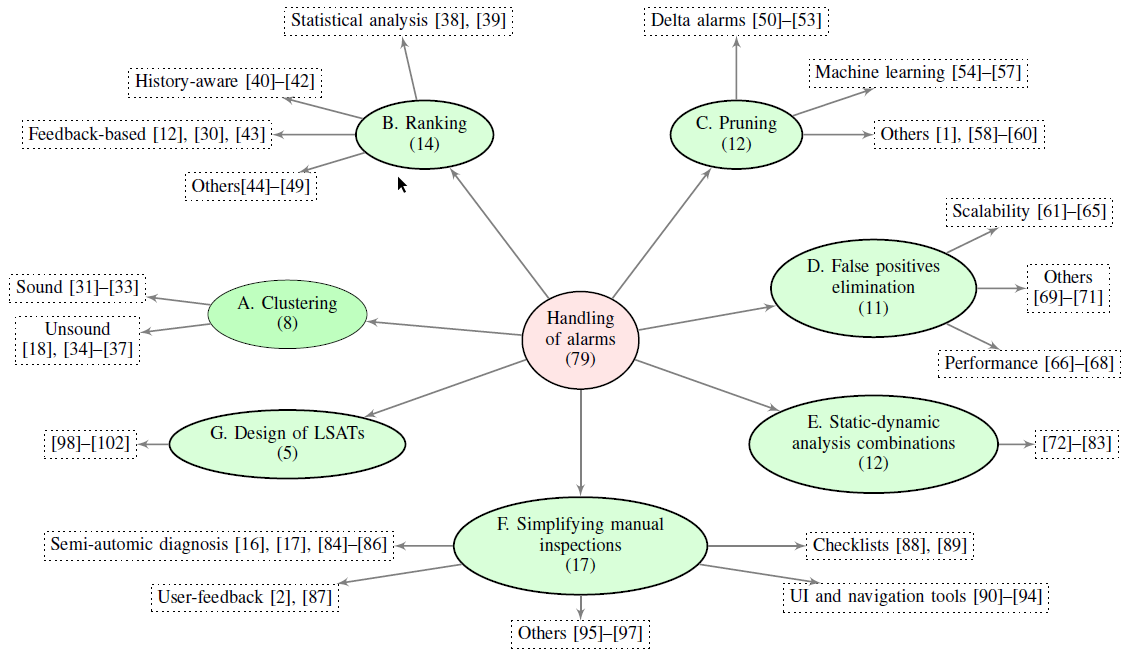
\includegraphics[scale=0.4]{./src/survey_sa_categories.png}
         \caption{Summary of the approaches}\label{survey:categories}
     \end{subfigure}
 \end{figure}


\subsubsection{Comparative studies}

Heckman and Williams \cite{comparative_heckman} perform a comparative study of six alert ranking techniques on the \textit{Faultbench} dataset: (a) Actionable Prioritization models that are based on the assumption that alerts sharing a type/location are like to be all actionable or non-actionable, (b) Alert Type Lifetime models that prioritize alert types by their average lifetime (important alerts are fixed quickly), (c) Check 'n Crash that automatically generates unit test cases and checks if the test fails (alert is then considered actionable), (d) History-Based Warning Prioritization models that uses commit messages and code changes in the source code repository to prioritize alert types, (e) Logistic Regression models that are trained on thirty-three alert characteristics and predict the probability of an alert being actionable, (f) Systematic Actionable Alert Identification that collects a number of alert characteristics and tries to find the best subset of these characteristics and the best machine learning models that optimizes accuracy and precision.

On each of the three test projects of the benchmark, there is a different winner (based on accuracy), with Systematic Actionable Alert Identification and Logistic Regression models that generally perform better. There is also a trend where precision and recall decrease with the amount of analyzed revisions (70, 80 or 90\%). That can be explained by the fact that the balance between actionable and unactionable alerts is heavily shifted to the later. This trend can also be explained by the fact that these techniques can be better at identifying unactionable alerts than actionable alerts.


Allier et al. \cite{compare_framework} perform a comparison of different ranking algorithms based on their effort metric: average number of alerts to inspect to find an actionable one. They also focus on two other research questions, whether its better to rank alerts individually or alert types, and if there is a performance difference between statistical ranking methods and ad-hoc ones. They test six raking approaches ( six Java and Smalltalk systems): Aware, FeedbackRank and Z-Ranking which mainly use alert type and location, RPM that uses logistic regression with thirty-three alert characteristics, AlertLifeTime that prioritizes alerts on type and lifetime, and EFindBugs which prioritizes alert types based on their defect likelihood.

They found out that Aware and FeedbackRank perform significantly better than the other ranking approaches. In addition individual alert raking algorithms performed better than those that rank alert types. Also they did not find a clear distinction in performance between statistical and ad-hoc approaches.


 \subsection{Bug Prediction}

 Nagappan et al. \cite{mining_metrics} use code complexity metrics to predict the likelihood of \textit{post-release} defects for new entities (failures that occurred in the field six months after the release). Although, according to their findings, these metrics are correlated to failure prone entities, there is no universal set of metrics that produces the best results. As a consequence, principal component analysis is used to choose the optimal set of features for a particular project. Information from bug databases and historical data is used to select the appropriate metrics.

 By analyzing a set of five large scale projects, they discovered the following results: (a) for each project a set of metrics can be found that correlates with post-release defects, (b) there is no single et of metrics that fits all projects, (c) predictors build using \textit{PCA} are useful for building regression models that predict post-release defects, (d) predictors are only accurate when obtain from the same or similar projects.

 This approach can be generalized to predict arbitrary measures of quality, as long as we can extract the right information from the project's history. The general workflow is the following: decompose system in entities, build a function that assigns a quality measure to an entity, have a set of metrics and a metric functions that assigns a value to each entity, determine correlation of metrics to the quality measure and use PCA to select the most relevant set, use the principal components to predict quality of new entities.

 % \begin{figure}[H]
 %     \centering
 %     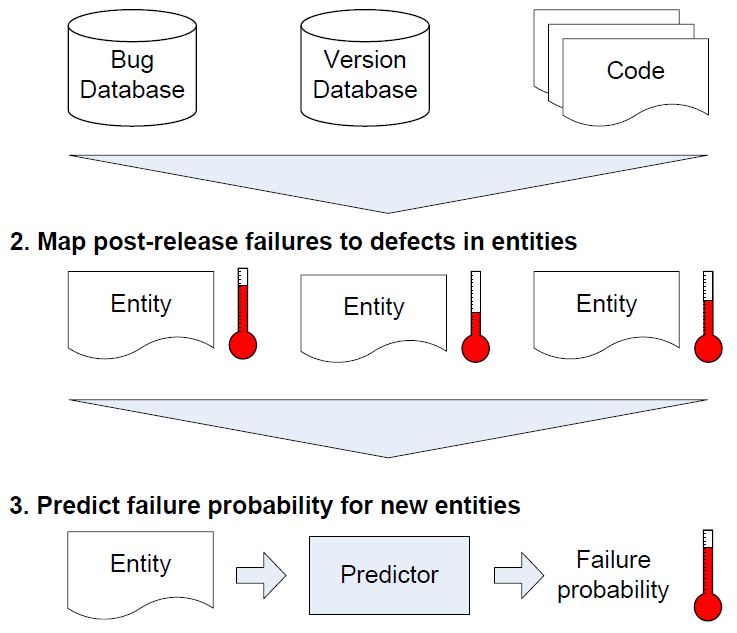
\includegraphics[scale=0.3]{./src/mining_metrics_overview.png}
 %     \caption{Some of the features considered for building the models}\label{mining:overview}
 % \end{figure}

 \begin{figure}[H]
     \begin{subfigure}{.5\textwidth}
         \centering
         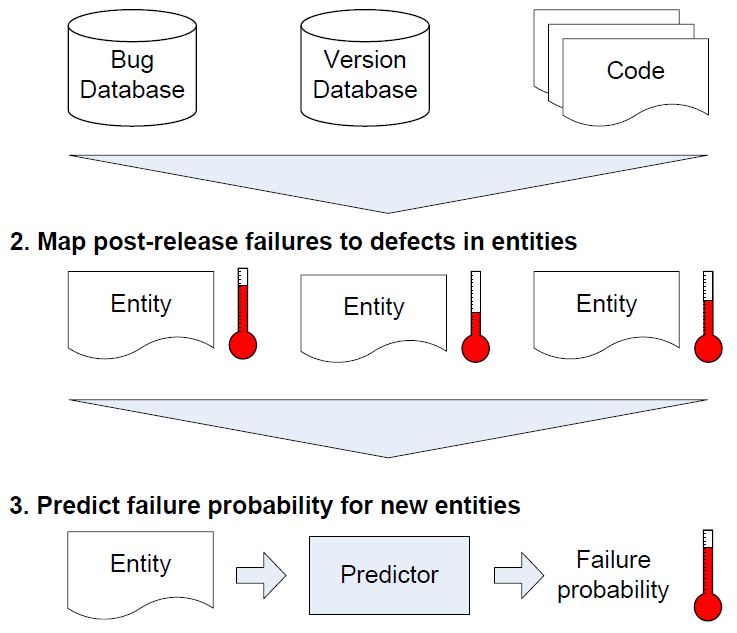
\includegraphics[scale=0.3]{./src/mining_metrics_overview.png}
         \caption{Workflow for predicting defects on new entities}\label{mining:overview}
     \end{subfigure}%
     \begin{subfigure}{.5\textwidth}
         \centering
         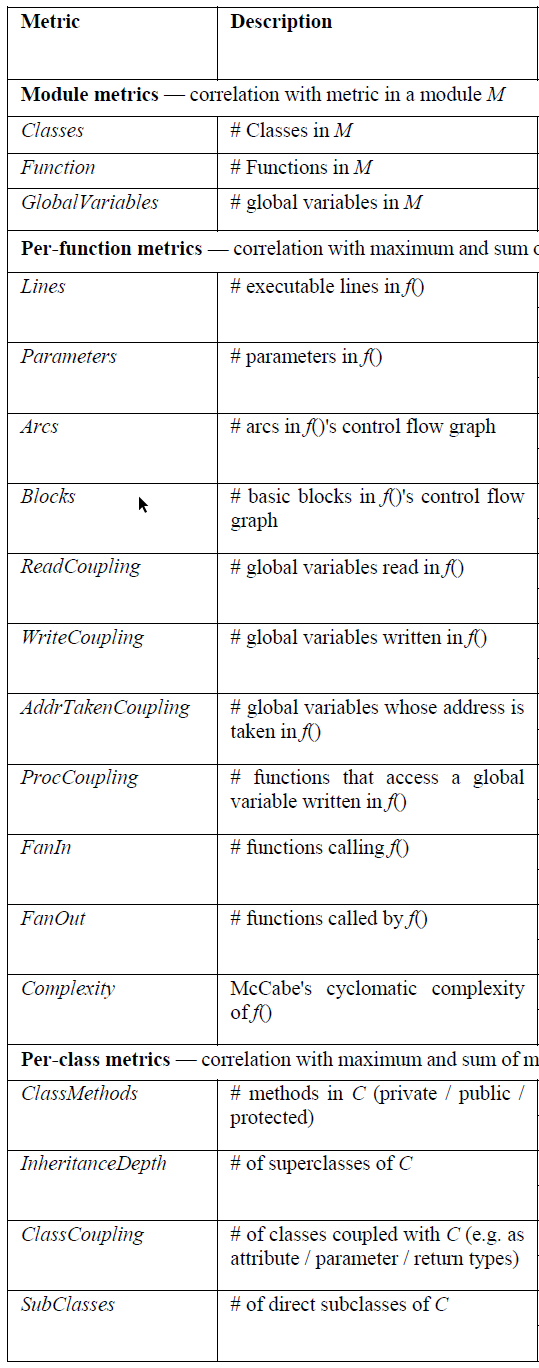
\includegraphics[scale=0.2]{./src/mining_metrics_metrics.png}
         \caption{The set of complexity metrics considered}\label{mining:metrics}
     \end{subfigure}
 \end{figure}


 Giger et al. \cite{prediction_method} present bug prediction models at method level. In comparison to previous file or module level techniques, this increases the granularity of the prediction and thus reduces manual inspection (developers don't have to inspect a whole file). 

 The models are based on source code metrics that are applicable on method level (\cref{method_prediction:metrics}) while change metrics are based on fine-grained operations extracted from AST comparisons (tree edit operations needed to transform one AST into the other, combined with semantic information from the source code, \cref{method_prediction:ast}).

 By using an extensive test set of multiple open source Java projects and by labeling each method as bug-prone or not bug-prone (using historical VCS data) they were able to measure the efficacy of different classifiers. The classifiers were trained with both source and change metrics and each separately. The source metrics alone performed significantly worse than the other two and suffer from low precision values (around \%50). The change metrics (combined or not with the source ones) perform significantly better (> 80 \% precision) and the type of classifier does not significantly affect the results (\cref{method_prediction:results}).

 \begin{figure}[H]
     \begin{subfigure}{.5\textwidth}
         \centering
         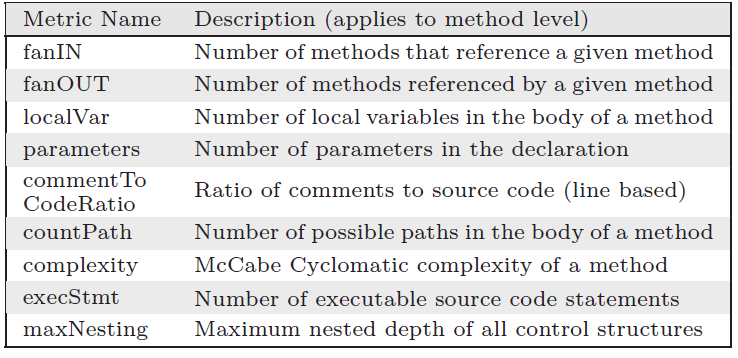
\includegraphics[scale=0.3]{./src/method_prediction_metrics.png}
         \caption{Method level metrics used for prediction}\label{method_prediction:metrics}
     \end{subfigure}%
     \begin{subfigure}{.5\textwidth}
         \centering
         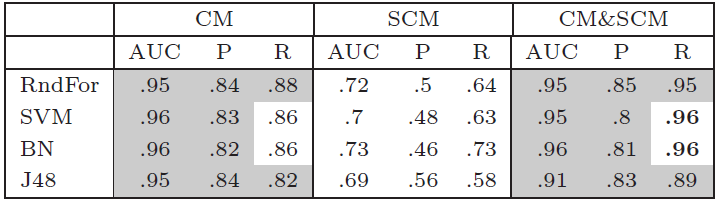
\includegraphics[scale=0.4]{./src/method_prediction_results.png}
         \caption{Precision, recall and AUC results for the metric sets}\label{method_prediction:results}
     \end{subfigure}\\
     \begin{subfigure}{\textwidth}
         \centering
         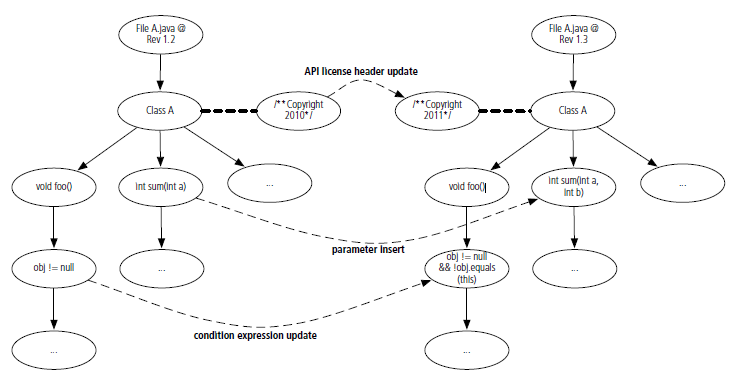
\includegraphics[scale=0.4]{./src/method_prediction_ast.png}
         \caption{Fine grained code changes extracted from AST comparisons}\label{method_prediction:ast}
     \end{subfigure}  
 \end{figure}


 Wang et al. \cite{predict_deeplearning} leverage deep learning to automatically learn semantic features from source code. The aim is to apply this knowledge into defect prediction, which traditionally uses syntactic features to build the models. In order to make accurate prediction, the features need to be discriminative, but traditional features cannot distinguish code regions with different semantics (see for example \cref{deeplearning:example}).

 A Deep Belief Neural Network is used to learn the semantic features from input vectors that contain tokens extracted from the AST's (code is parsed into tokens, tokens are then mapped into integers, which then form the vectors). Three main categories of AST nodes are extracted: a) nodes of method invocations and class instance creations, b) declaration nodes, c) and control flow nodes (see \cref{deeplearning:workflow} for the general workflow).

 To handle noise in data, the edit distance between the token sequences along with the \textit{Closest List Noise Identification} approach is used (compare instance label against its k-nearest neighbors). Additionally, infrequent tokens are filtered out of the training process.

 The DBN is tested against models trained with traditional features and models trained with the AST nodes. As can be seen from \cref{deeplearning:results}, the DL approach outperforms the traditional methods, with an average improvement in precision and recall of 14\% and 11\% respectively.

 \begin{figure}[H]
     \begin{subfigure}{1\textwidth}
         \centering
         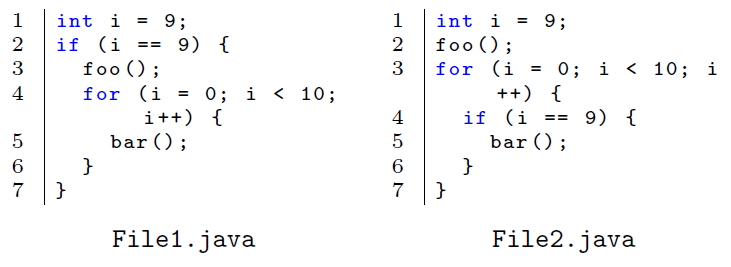
\includegraphics[scale=0.5]{./src/deeplearning_example.png}
         \caption{Example of programs with same syntax (tokens) but different semantics}\label{deeplearning:example}
     \end{subfigure}\\
     \begin{subfigure}{\textwidth}
         \centering
             \makebox[\textwidth]{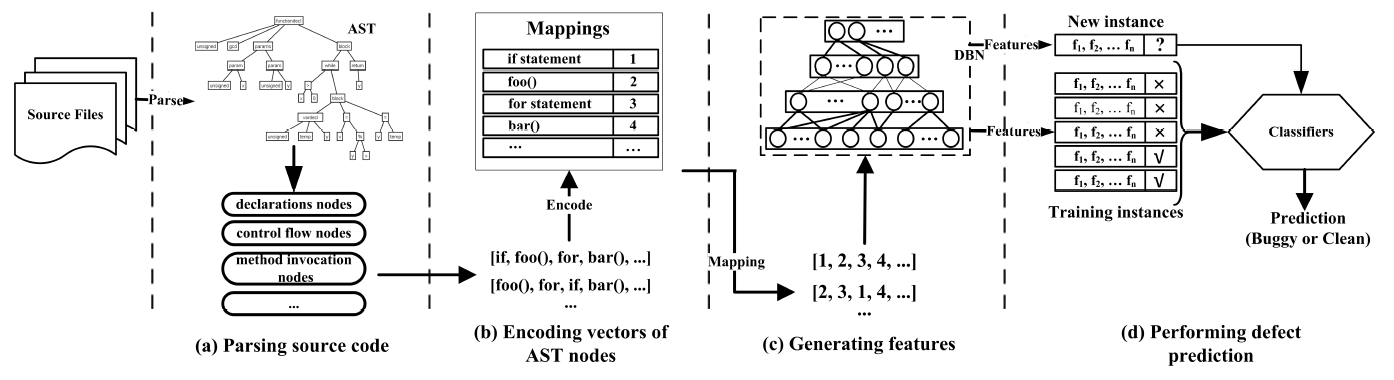
\includegraphics[scale=0.5]{./src/deeplearning_workflow.png}}%
         \caption{Workflow for the semantic learning process}\label{deeplearning:workflow}
     \end{subfigure}\\
     \begin{subfigure}{1\textwidth}
         \centering
         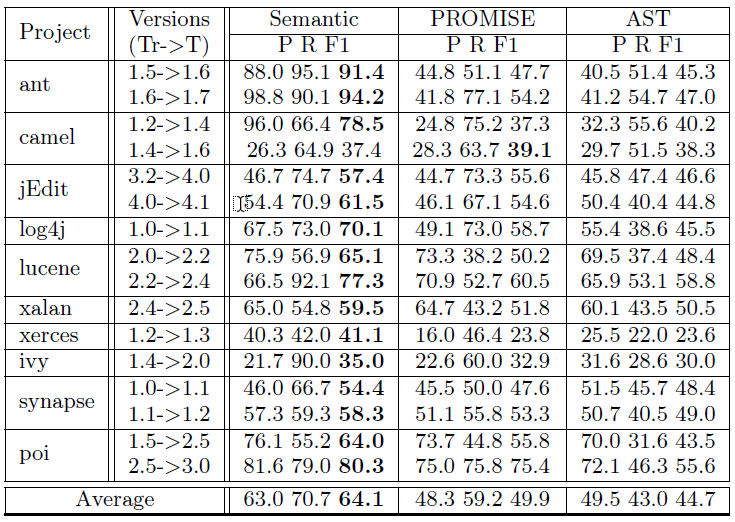
\includegraphics[scale=0.4]{./src/deeplearning_results.png}
         \caption{Precision, recall and F1 score for semantic vs syntactic features}\label{deeplearning:results}
     \end{subfigure}
 \end{figure}


 Yang et al. \cite{dl_jit_prediction} propose a deep learning technique to detect defect-prone changes (just-in-time defect prediction, i.e. inside commits). The advantage of this granularity is that there is a smaller amount of code to check and that it is easy to decide which developer should fix a bug (the one who committed the code). They use a two phase approach: a feature selection phase and a machine learning phase.

 The feature selection phase is to decide the best set of features to use to train the model. The data is pre-processed to in two steps: data is first normalized and then random under-sampling is used to balance the categories of buggy or not buggy changes. Since in logistic regression each feature is calculated independently, new features cannot be created by combining existing ones. For that reason, they leverage \textit{Deep Belief Networks} to generate a more expressive feature set. 

 The logistic regression model is trained with the new feature set and evaluated with a cost effectiveness measure defined as the percentage of bugs that can be discovered by inspecting the top (most relevant) 20\% lines of code. On average 50\% of bugs can be found in the top 20\% LOC, and the feature processing step helps logistic regression achieve better results than previous approaches (\cref{dl_jit:results}).

 \begin{figure}[H]
     \centering
     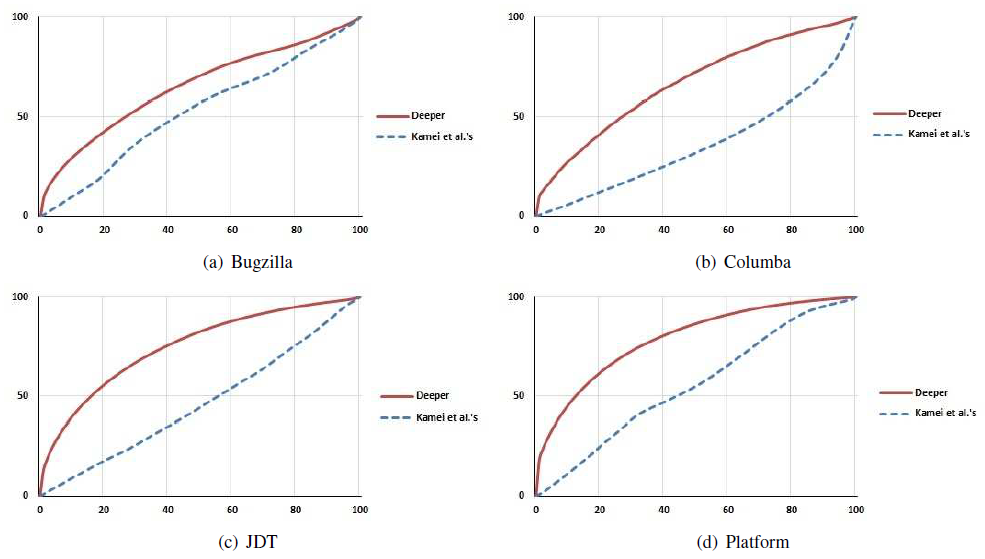
\includegraphics[scale=0.5]{./src/dl_jit_results.png}
     \caption{Improvements over classic logistic regression approach}\label{dl_jit:results}
 \end{figure}



 \subsection{Static Analysis tools in practice}

 Beller et al. \cite{analysis_sa_usage} conduct a large scale evaluation of how SA tools are used in practice in open-source systems. They study the prevalence of SA tools, their configurations and how they evolve.

 By performing a survey on a 36 open-source projects, they found out that most of them used SA tools, with a relevant subset using more that one (\cref{sa_analysis_survey:usage}). Although, most of them run the tools sporadically and without enforcing them.

 A configuration file of a SA tool, shows what rules developers deem important (enable), and what they do not deem important (disabled, perhaps because of a high false positives rate). The contents of a configuration file are hence an important indicator of how developers use SAs and how well the tool’s default settings reflect its use.

 In the analyzed projects, most enabled rules belong to the maintainability category, and only 35\% of the enabled rules belong to a functional category. Both the majority of actively enabled and disabled rules are maintainability-related.

 Most configurations change or reconfigure rules from the default configuration, but typically only one rule. Most changes are small, and a third of them happen in the first week of creation of the configuration. Also, most configuration files never change (\cref{sa_analysis_survey:changes}).

 \begin{figure}[H]
     \begin{subfigure}{1\textwidth}
         \centering
         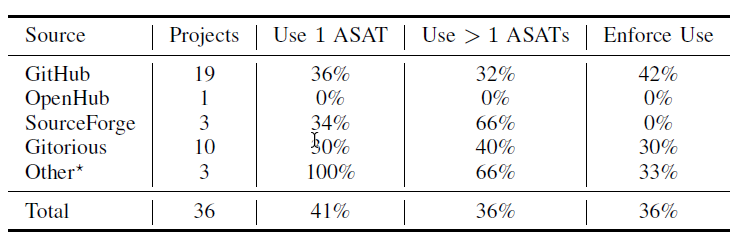
\includegraphics[scale=0.4]{./src/sa_analysis_survey_usage.png}
         \caption{Survey results of 36 open-source systems using SA tools}\label{sa_analysis_survey:usage}
     \end{subfigure}\\
     \begin{subfigure}{1\textwidth}
         \centering
         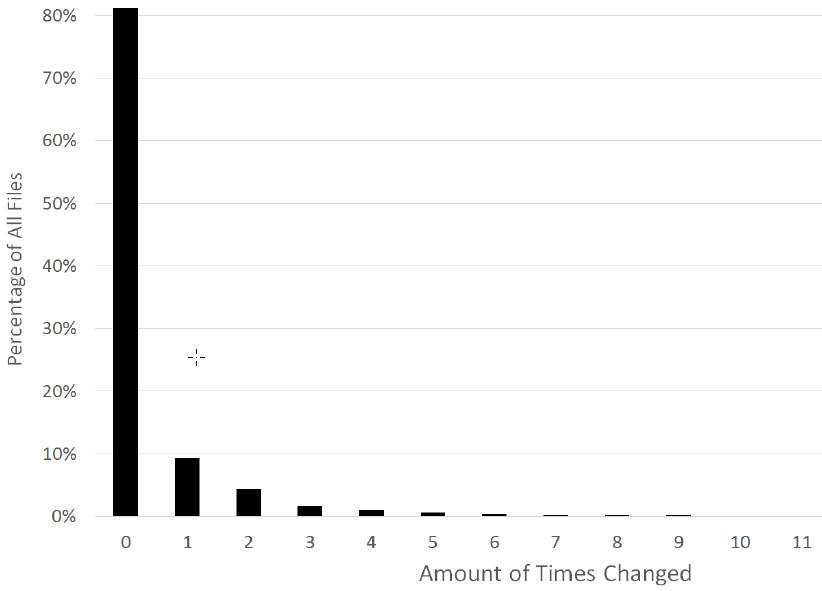
\includegraphics[scale=0.4]{./src/sa_analysis_survey_changes.png}
         \caption{Changes in configuration of SA tools}\label{sa_analysis_survey:changes}
     \end{subfigure}
 \end{figure}


 Imtiaz et al. \cite{how_act_sa} analyze the SA usage of five large open-source systems (the tool is \textit{Coverity}). They study the amount of actionable alerts, time for fixing alerts and the size of fixes.

 They discover that 80\% of alerts belong to 20\% of the alert types and that the actionability rate varies from 27\% to 49\% depending on the project (\cref{how_use_sa:actionable}). Also in the case of actionable alerts, 20\% of the types causes 80\% of the actionable alerts.

 The median lifespan of actionable alerts varies between projects, ranging from 36 to 245 days, and the complexity of code changes is generally low. This means that developers generally take a long time to fix the alerts despite the fixes being low in complexity.

 To increase the developer interaction with SA tools they suggest two solutions: (a) prioritizing the most critical alerts and (b) providing an estimate for the fix effort.

 \begin{figure}[H]
     \begin{subfigure}{1\textwidth}
         \centering
         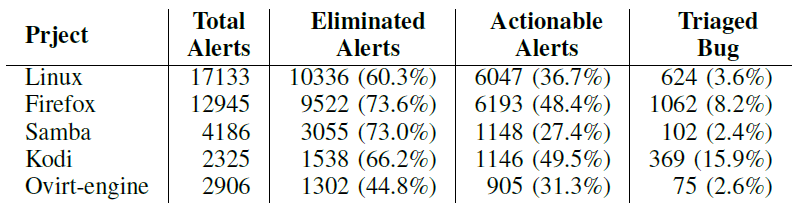
\includegraphics[scale=0.4]{./src/how_use_sa_actionable.png}
         \caption{Actionability results for total alerts}\label{how_use_sa:actionable}
     \end{subfigure}\\
     \begin{subfigure}{1\textwidth}
         \centering
         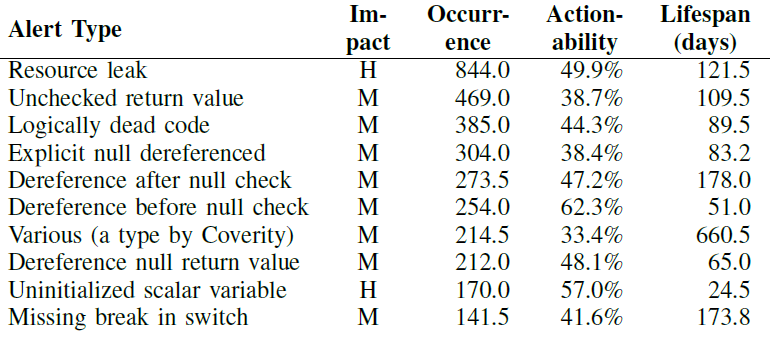
\includegraphics[scale=0.4]{./src/how_use_sa_topalerts.png}
         \caption{Top 10 alert occurrences for C/C++}\label{how_use_sa:top}
     \end{subfigure}
 \end{figure}


 Habib and Pradel \cite{how_many_bugs} study how many of all real-world bugs static bug detectors find. The results of their study show that: (a) static bug detectors find a non-negligible amount of all bugs, (b) different tools are mostly complementary to each other (see \cref{how_many_bugs:partition}), and (c) current bug detectors miss the large majority of the studied bugs.

 The three bug detectors together reveal 27 of the 594 studied bugs (4.5\%). Some of the missed bugs could have been found by variants of the existing detectors, while most of them are domain-specific problems that do not match any existing bug pattern that the SA tool have. By manually analyzing a small subset of 20 bugs, 14 of them were domain-specific and not related to any pattern supported by the checkers, while 6 of them were near-misses that could have been detected with a more powerful variant of the tool.

 They also found that the majority of bug fixes is limited in size and that most bugs are clustered on a small percentage of files (\cref{how_many_bugs:fixsize}).

 \begin{figure}[H]
     \begin{subfigure}{1\textwidth}
         \centering
         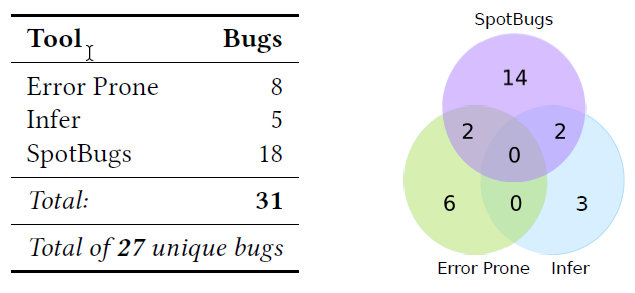
\includegraphics[scale=0.4]{./src/how_many_bugs_partition.png}
         \caption{Distribution of found bugs per tool}\label{how_many_bugs:partition}
     \end{subfigure}\\
     \begin{subfigure}{1\textwidth}
         \centering
         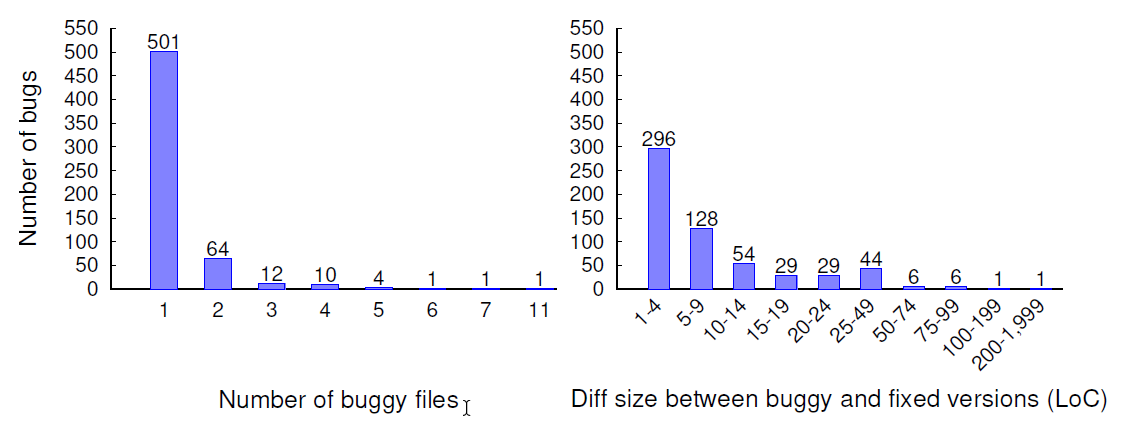
\includegraphics[scale=0.4]{./src/how_many_bugs_fixsize.png}
         \caption{Bugs/file and lines/bugfix}\label{how_many_bugs:fixsize}
     \end{subfigure}
 \end{figure}


 Sadowski et al. \cite{sa_google} provide an overview of the process that Google underwent to increase the developer interaction with SA tools. They list a number of shortcomings that hinder large scale adoption of such tools and suggest solutions that proved effective in their company. 

 The main reasons developers ignore of lose faith in SA tools are: (a) \textbf{no integration in workflow} (most important reason), (b) non actionable warnings, (c) reported bugs do not manifest in practice, (d) suggested bug is too risky/expensive to fix, (e) warnings are not understood.

 Google switched from the dashboard based \textit{FindBugs} tool (whose warnings were mostly ignored for two main reasons: developers lost faith because of false positives or alerts that were not important, and because the warnings came to late in the development workflow), to another better integrated approach.
 According to their findings, reporting issues sooner is better: moving as many checks into the compiler is the way to go. When possible, fixes are suggested or carried out automatically. A second place to show alerts that relate to high impact bugs, is the code review platform (for alerts with no simple fix). Code review is also a good context for reporting relatively less-important issues like stylistic problems or opportunities to simplify code.

 Another key point in making SA tools more valuable for the developers, is integrating their feedback, whether they accept or not the alerts proposed by the tool (for ex. adding a button for each alert \textit{Useful/Not Useful}).
 An additional workflow integration point is \textit{gating commits}: blocking a commit when a check fails (used for check with a low false positive rate).


% \subsection{Available tools}
% Open source tools found:
% \begin{itemize}
%     \item Infer
%     \item CppCheck
% \end{itemize}

% \subsection{Ideas?}
% \begin{itemize}
%     \item \textbf{Feasibility study}: combining different techniques (\cite{survey_approaches}). Pipelining or parallel?
%     \item mine bug messages / fixes to extract useful information?
%     \item use \cite{mining_metrics} to predict actionable warnings
%     \item lightweight local (file level?) execution likelihood
%     \item z-ranking or weighted warnings for cpp core guidelines
%     \item use ignore commands found in code for pruning future warning reports
%     \item see \cite{predict_deeplearning} introduction for a list of feature selection (also links to interesting papers)
%     \item To prune noisy data: mislabeling data detection approach Closest List Noise Identification (CLNI).
%     \item deep learning to classify warnings
%     \item single rule classifiers?
%     % \item consider the psycological aspect (coverity paper and \cite{sa_google})
%     \item when using multiple tools, consider the warning mapping (\cite{analysis_sa_usage}, \cite{multiple_ensemble}, \cite{multiple_classification}).
%     \item identify most relevant alert categories (80\% of actionable alerts come from 20\% of the types)
%     \item provide estimate for the fix?
%     \item less critical warnings as code review (+button, useful or not)
%     \item different checkers can be more useful for different teams
%     \item age of files is important!!! -> incremental detection
%     \item \textbf{mine patterns in ignored alerts?}
%     \item which context information to extract? first order logic approach \cite{incremental_sa} or sat tools?
%     \item can slicing be used?
%     \item differential changes as features?
%     \item cache locality?
%     \item check if pdg of clang can be useful
%     \item z ranking - core guidelines - based on file level (absence of warning -> successful check)
%     \item correlation tests between errors/warnings and exec likelihood/method bug score
%     \item use clang info on bug related lines
%     \item CLUSTER ALERTS!!!
%     \item \textbf{ignore closed alerts by clang-diagnostic-error}
%     \item fix number of authors
%     \item \textbf{consider the correlations between techniques}
%     \item use \textbf{clone information to cluster reports}
%     \item \textbf{CHECK WARNING AVERAGE LIFETIME: for remaining warnings unactionable if lifetime bigger than average}
% \end{itemize}


% \subsection{Acronyms}
% \begin{itemize}
%     \item SA - Static analysis
%     \item AA - actionable alert
%     \item AST - Abstract syntax tree
%     \item DL - Deep learning
% \end{itemize}
